\begin{frame}{Simple Linear Regression}
    \begin{figure}
        \centering
        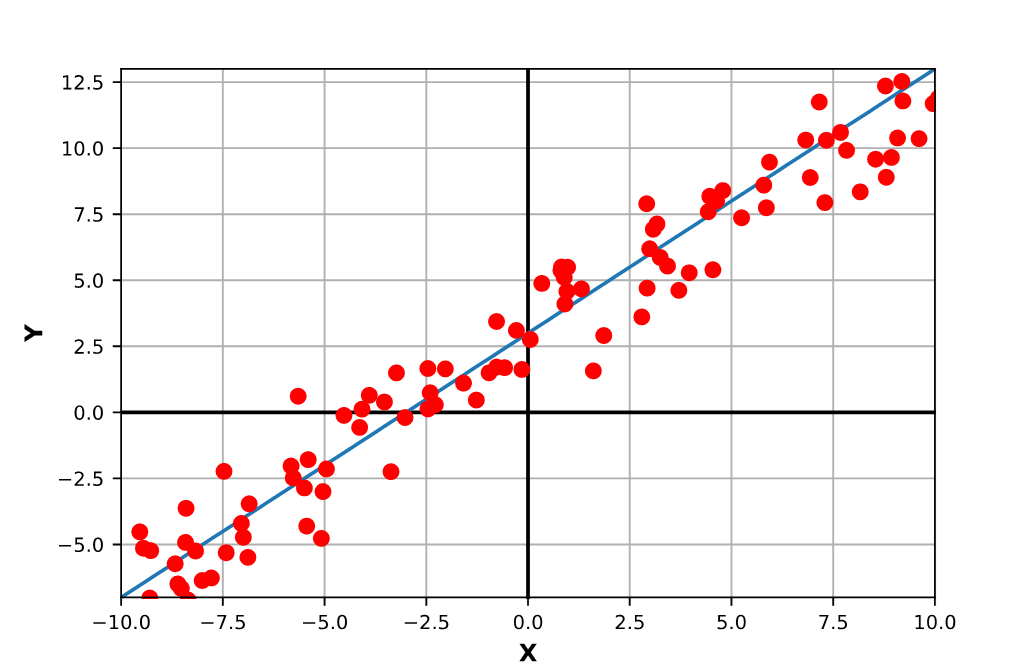
\includegraphics[width=0.5\textwidth]{images/linear-regression/linear-regression-5.png}
        \caption*{\small Model (\textit{Linear}): $Y = mX + b$ \hfill $\theta = \{m, b\}$}
    \end{figure}

    \begin{itemize}
        \item Y: Response Variable
        \item X: Covariate / Independent variable / Regressors
        \item m: slope
        \item b: bias
    \end{itemize}
\end{frame}


\begin{frame}{Simple Linear Regression}
    \begin{itemize}
        \item \textbf{Hypothesis:} $\hat{y}_i = mx_i + b$
        
        \item \textbf{Input:} data $(x_i, y_i), \ i \in \{1, 2, \ldots, N\}$
        \begin{itemize}
            \item (e.g., house size $x$ and price $y$)
        \end{itemize}
        
        \item \textbf{Goal:} learn values of variable $(m, b)$
    \end{itemize}
\end{frame}

\begin{frame}{Notation}
    \begin{itemize}
        \item Some clarification about the notation we will use for this course
    \end{itemize}

    \begin{center}
        {\Huge $X_i^{j, [k]}$}
    \end{center}

    \begin{itemize}
        \item $i$ is the index of the data, $j$ is the feature number, and $k$ is the power.
    \end{itemize}
\end{frame}

\begin{frame}{Solution Strategy for Solving the Problem}
    \begin{itemize}
        \item There are countless possible lines.
        \item We want a line which is in some sense the “average line” that represents the data.
        \item Any ideas as to how we can do it?
    \end{itemize}

    \begin{center}
        \href{https://i.imgur.com/A1tDy8G.gif}{
            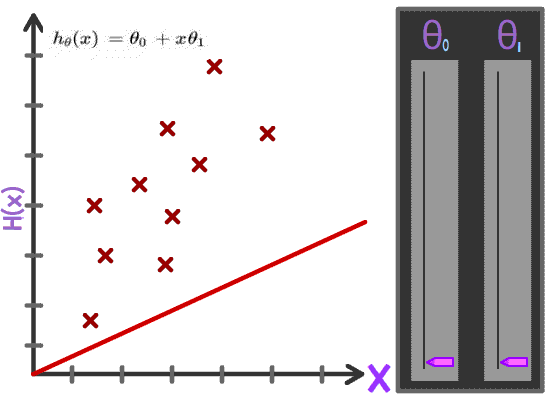
\includegraphics[width=0.6\linewidth]{images/linear-regression/linear-regression-6.png}
        }

        {\scriptsize Click the image to view the animated version.}
    \end{center}
\end{frame}

